\documentclass{sig-alternate}
\usepackage{graphicx}
\usepackage{url}
\usepackage{paralist}
\usepackage{listings}
\usepackage{caption}

% \DeclareUnicodeCharacter{B1}{\pm}
%% LANGUAGE      Markup definitions
\def\lstxml{
  \lstset{language=XML,
    keywordstyle=\ttfamily,
    identifierstyle=\ttfamily\bfseries, 
    % commentstyle=\color{Brown},
    stringstyle=\ttfamily,
    showstringspaces=false,
    columns=[l]flexible, %% , basewidth={0.5em,0.4em}
    escapeinside={(@*}{*@)},
    morekeywords={encoding,
      mrow,math,mfrac,mi,msqrt,mo,mn,span,nobr,img}
  }
}

\def\lstjs{
  \lstset{language=Java,
    keywordstyle=\ttfamily,
    identifierstyle=\ttfamily\bfseries, 
    % commentstyle=\color{Brown},
    stringstyle=\ttfamily,
    showstringspaces=false,
    columns=[l]flexible, %% , basewidth={0.5em,0.4em}
    morekeywords={cvox,Api,Math,defineRule}
  }
}

\def\lsttex{
  \lstset{language={[LaTeX]TeX},
    texcsstyle=*\bfseries,
    keywordstyle=\ttfamily,
    identifierstyle=\ttfamily\bfseries, 
    % commentstyle=\color{Brown},
    stringstyle=\ttfamily,
    showstringspaces=false,
    columns=[l]flexible, %% , basewidth={0.5em,0.4em}
    moretexcs=intertext,
    morekeywords={sum,Sigma}
  }
}

\newcommand\ednote[1]{\typeout{There is still a note!!!}%
  {\bf EDNOTE: #1}}

\newcommand\edbf[1]{\typeout{There is still an editor's note!!!}%
  \textbf{EDNOTE: #1}}


\begin{document}
\title{Accessibility to Scientific Material:\\ The Case of Speaking Math}
\numberofauthors{2} %  in this sample file, there are a *total*

\author{
% You can go ahead and credit any number of authors here,
% e.g. one 'row of three' or two rows (consisting of one row of three
% and a second row of one, two or three).
%
% The command \alignauthor (no curly braces needed) should
% precede each author name, affiliation/snail-mail address and
% e-mail address. Additionally, tag each line of
% affiliation/address with \affaddr, and tag the
% e-mail address with \email.
%
% 1st. author
  \alignauthor Volker Sorge\titlenote{This work was done while the author spent a
    sabbatical at Google,
    Inc., Mountain View, CA, USA.}\\
  \affaddr{School of Computer Science}\\
  \affaddr{The University of Birmingham, UK}\\
  \email{V.Sorge@cs.bham.ac.uk}
% 2nd. author
\alignauthor
Charles Chen, T.V. Raman, David Tseng\\
       \affaddr{Google, Inc.}\\
       \affaddr{Mountain View, CA, USA}\\
       \email{\{clchen|raman|dtseng\}@google.com}
}


\maketitle 
\begin{abstract} 
  As the traditional methods of publishing and teaching in the
  STEM subjects are being progressively replaced by the provision
  of web-based content, ensuring full accessibility to this
  material for visually impaired users is of paramount importance
  for inclusive education. The text to speech translation of
  content for which well defined markup languages exists such as
  mathematics is a non-trivial problem. In this paper we present
  our efforts of making the speech translation of mathematical
  formulas a first class citizen in a general screen reader. We
  describe the ChromeVox screen reader and demonstrate how its
  features enable us to provide text to speech translation for
  web-based mathematical content. These features allow us to
  translate formulas given in a variety of formats into uniform
  spoken utterances exploiting ChromeVox's ability to handle
  alternative representations of DOM elements. This also allows
  us to customize aural rendering of mathematics both by using
  semantically enriched representations and employing flexible
  and adaptable speech rules. To further aid understanding of the
  math we exploit ChromeVox's idea of letting users engage with
  content on different levels of granularity to enable
  interactive exploration of complex mathematical formulas.
\end{abstract}
\category{H.5.2}{User Interfaces}{Voice I/O}
%A category including the fourth, optional field follows...
\category{H.5.4}{Hypertext}{Navigation, User Issues}

% \terms{}

\keywords{screen reader, mathematics, ChromeVox}

\section{Introduction}\label{sec:intro} As we move away from the traditional
methods of publishing and teaching to the provision of web-based content, more
and more scientific literature and teaching material in the STEM subjects
becomes available online. This material can range from traditional articles
containing mathematical formulas and scientific diagrams to highly interactive
web pages often exploiting novel media formats such as dynamic diagrams or
simulations. Ensuring full accessibility to this material for users that rely
primarily on voice output from their computer becomes a challenging
problem. Already the text to speech translation of fairly conventional
scientific content like mathematical formulas, which contain rich structure and
for which a well defined markup language exists, is non-trivial.


\ednote{Some related work here.}

In this paper we report on our effort to integrate the basic support
for voicing mathematical content on the web into the ChromeVox screen
reader. 



As an example we consider the quadratic formula:
\begin{equation}
  \label{eq:quadratic}
  x=\frac{-b \pm \sqrt {b^2-4ac}}{2a}
\end{equation}


We shall present some of the main challenges to making maths
on the web accessible, where it is given in a variety of ways and
formats. We shall outline the rule based approach we have pursued and
how it fits with ChromeVox's philosophy to enable users to explore
content at different levels of granularity. It has led to an
implementation of a flexible speech rule engine that allows to
customize the reading experience along several axes and that also
provides an API for easy adaptation to specialized content by users
and web site authors.

\section{Mathematics on the Web}
\label{sec:math}

Mathematical formulas on web pages can be represented in their own specialized
markup language, MathML~\cite{MathML3}. But although MathML is officially part
of the HTML5 standard~\cite{HTML5}, not all major browsers also implement MathML
rendering, hence support displaying formulas included in pure MathML on web
pages is sketchy. Consequently in reality mathematics on the web comes in a
variety of flavors. One can identify predominant three ways in which
mathematical content is currently given on the web:
\begin{enumerate}
\item Pure MathML markup: this relies on the user viewing the
  page with a browser that renders MathML.
\item Rendered with MathJax: the web page author ensures that mathematical
  content is rendered client-side independent of the user's browser by including
  the third party MathJax library in the page. Formulas can be given in several
  different markup languages.  and relying on the third party that renders
  mathematical content client side.
\item Pre-rendered images: Content is ensured to display correctly, by including
  images of formulas in the web page. The original markup from which the content
  was originally rendered is often given in an attribute of the image tag.
\end{enumerate}

In order to enable access to the majority of mathematics that can be found on
the web today, one has to provide text-to-speech support for all of the above
formats, which we shall briefly sketch the remainder of this section.

\subsection{MathML}
\label{sec:mathml}

MathML is a specialized markup language that was developed with the expressive
purpose of representing mathematics. Ordinarily it comes in two flavors:
presentation MathML and content MathML. The former is a markup language geared
towards adequately displaying mathematical formulas thus playing a role of web
documents similar to the one of {\LaTeX} for printed documents.  Contrary,
content MathML aims to serve also as a meaningful exchange format between
mathematical software systems by providing markup that allows to express
semantic meaning of mathematical expressions. As there is still very little
support for content MathML we concentrate here on presentation MathML only.
  
\begin{figure}[t!]
  \begin{center}
    \leavevmode
    \lstxml\small
\begin{lstlisting}
<math xmlns="http://www.w3.org/1998/Math/MathML">
  <mstyle displaystyle="true">
    <mi>x</mi>
    <mo>=</mo>
    <mfrac>
      <mrow>
        <mo>&#x2212;</mo>
        <mi>b</mi>
        <mo>&#x00B1;</mo>
        <msqrt>
          <msup>
            <mi>b</mi>
            <mn>2</mn>
          </msup>
          <mo>&#x2212;</mo>
          <mn>4</mn>
          <mi>a</mi>
          <mi>c</mi>
        </msqrt>
      </mrow>
      <mrow>
        <mn>2</mn>
        <mi>a</mi>
      </mrow>
    </mfrac>
  </mstyle>
</math>
\end{lstlisting}
    \caption{MathML representations of~\ref{eq:quadratic}.}
    \label{fig:quadratic-mml}
  \end{center}
\end{figure}

Presentation MathML provides markup for the most common layout elements
encountered in mathematics, such as sub- and superscripts, fractions, square
roots etc.  In addition it provides markup to define mathematics specific styles
or spacing, as well as specialised attributes such as for fonts, accents, etc.
Fig.~\ref{fig:quadratic-mml} presents our example the quadratic
formula~\ref{eq:quadratic} in MathML markup. Here the tags \texttt{mi},
\texttt{mn}, and \texttt{mo} markup identifiers, number, and operators,
respectively, while layout elements fraction, square root and superscript are
enclosed in the elements \texttt{mfrac}, \texttt{msqrt}, and \texttt{msup}. The
\texttt{mrow} tag allows the horizontal combination of a string of elements, in
case they need to be combined to a single node as in the case of the two
arguments for the fraction tag \texttt{mfrac}.

MathML is part of the specification for the HTML5 standard~\cite{HTML5}, where
it lives in its own name space. By extension it is also part of the ePub3
standard~\cite{epub3} and consequently one can anticipate that future
implementations of these standards with include native rendering of MathML
content. However, in the current situation only few browsers and epub readers
support MathML and rendering is either achieved by specialist browser plugins or
by third party libraries.


\subsection{MathJax Rendering}
\label{sec:mathjax}

MathJax is a JavaScript display engine~\cite{MathJax2.2} that consistently
renders mathematical expressions in all browsers. It handles a number of input
formats and translates them into simple HTML markup that visually renders a math
expression in a browser, regardless of whether it supports MathML.  Thus the
basic goal is to shift control on whether and how formulas are displayed to the
content author, by allowing them to include JavaScript in web pages that calls
MathJax via a content distribution network to enable client side rendering of
math expressions.

\begin{figure*}[t!]
%\begin{minipage}[t!]{\textwidth}
  \begin{center}
    \leavevmode
    \lstxml\small
    \lstinputlisting{mathjax.xml}
%    \captionof{figure}{MathJax representations of~\ref{eq:quadratic} from
    \caption{MathJax representations of~\ref{eq:quadratic} from
      \protect\url{en.wikipedia.org/wiki/Quadratic_equation}.}
    \label{fig:quadratic-mj}
    \leavevmode
    \lstxml\small
\begin{lstlisting}
<img class="tex" 
      alt="x=\frac{-b \pm \sqrt {b^2-4ac}}{2a}" 
      src="//upload.wikimedia.org/math/3/c/a/3ca857f705daba6b9e6e6d3ccad7990f.png" />
\end{lstlisting}
\caption{Image markup for~\ref{eq:quadratic} from 
  \protect\url{en.wikipedia.org/wiki/Quadratic_equation}.}
\label{fig:quadratic-img}
  \end{center}
\end{figure*}

An authors can then include formulas directly into a web page either as MathML
markup or as {\LaTeX} or AsciiMath~\cite{asciimath}. During the rendering
process MathJax replaces this markup with HTML elements that explicitly specify
vertical and horizontal spacing, drawing of lines and special elements such as
radices, and placement of character in web fonts.  This has not only the
advantage that the generated markup is portable between browsers, but also that
expressions rendered with MathJax are fully scalable.  But since the rendered
expressions that MathJax injects into the DOM is primarily aimed at visual
display, it is a less straightforward translation of the mathematical expression
it models.

As an example Fig.~\ref{fig:quadratic-mj} shows part of the MathJax markup for
equation~\ref{eq:quadratic}. While it is clearly more cluttered than its MathML
counterpart in Fig.~\ref{fig:quadratic-mml}, there are nevertheless some obvious
resemblances. The expression effectively consists of two types of \texttt{span}
elements:
\begin{inparaenum}[(a)]
\item Those with a single style attribute that are exclusively display elements.
\item Those with a additional class attributes and id that generally mirror the
  composition of the corresponding MathML expression.
\end{inparaenum}
As we can observe in our example, the latter type of elements maintains the
structure of the MathML expression, and this regardless of the original source
of the formula. Indeed MathJax always maintains an internal MathML
representation of a mathematical formula, even if translated from {\LaTeX} or
AsciiMath, a fact that we shall exploit in Sec.~\ref{sec:alternative}.


\subsection{Hidden Markup}\label{sec:images}

Traditionally mathematical formulas would be embedded into web content using
images generated from documents that were previously generated with systems
specializing on rendering mathematics, for example, {\LaTeX}. And despite the
obvious drawbacks of having content in images, such as lack of scalability, this
method is still an option that is chosen by many major web sites containing
mathematical content (e.g., Wikipedia~\cite{wikipedia},
MathWorld~\cite{mathworld}), to provide content consistently at reliable
performance, independent of third party libraries.  While the mathematics given
in image form is effectively inaccessible, the original source from which a
formula has been generated is often given in form of alternative text attribute
of the image tag.  For instance, in the case of Wikipedia, most of the
mathematics images have alternative text provided in \LaTeX, whereas Mathworld
contains AsciiMath markup.  The case of our example is given in
Fig.~\ref{fig:quadratic-img} the quadratic equation is loaded as a PNG images,
while the hidden markup is given in the original \LaTeX
\verb+x=\frac{-b \pm \sqrt {b^2-4ac}}{2a}+



This form of hidden markup can then be displayed in
text-only browsers or used for copy-and-paste operations. 
In ChromeVox we exploit hidden markup as well, to ensure a consistent
screen reading experience of all mathematical content on the web.  In particular,
we rely on the MathJax library to translate hidden markup into a MathML
representation that we can speak instead. We describe in detail the treatment of
alternative representations in Sec.~\ref{sec:alternative}.




\section{ChromeVox}
\label{sec:chromevox}

ChromeVox is a screenreader that has been built with the aim to make rich web
applications accessible to visually impaired users. ChromeVox runs inside the
Chrome browser where it can be installed as an extension and it is the default
screenreader for Chrome OS. Therefore, it uses exclusively the HTML document
object model (DOM) to communicate with web applications without the need to user
an accessibility API provided by the underlying operating system.

With the advancements of the web programming model and in particular the ease
with which complex interaction layers can be build using HTML, CSS and
JavaScript web pages do no longer just contain but resemble fully fledged
applications more akin to traditional desktop programs. As a consequence
traditional linear navigation is no longer sufficient to allow users to explore
and comprehend web content in a reasonable way.

ChromeVox aims to support effective navigation of complex web content by giving
the user the means to engage with content on multiple layers. This is
implemented via an architecture that makes it possible to customize the screen
readers behavior along four axes which allows to adapt the screenreader
flexibly to specialized content. In detail ChromeVox can be parameterized by 
\begin{enumerate}[(1)]
\item segmenting the DOM into different \emph{granularities},
\item enabling different ways of interactively \emph{walking content},
\item customizing content description by parameterizing a \emph{speech output},
\item enabling efficient navigation by allowing the use of \emph{alternative
    representations} for DOM elements.
\end{enumerate}
In the remainder of this section we will explain these four axes in more detail.


\subsection{Axis 1: Granularities}
\label{sec:ax1}

Granularities are the primary means to allow a user to engage with content at
their choice of detail. The main purpose of a granularity is to segment the DOM
into units between which the user can navigate interactively.

In practice, a granularity defines what is regarded as a leaf node in the
DOM. Fig.~\ref{fig:granularity} schematically depicts the idea of different
granularities. The content of the leaf node is then the smallest chunk that is
translated into an utterance and sent to the TTS.

\begin{figure}[ht!]
  \begin{center}
    \leavevmode
    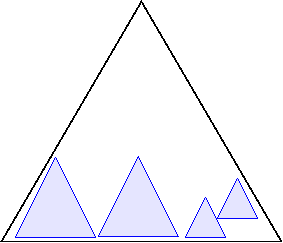
\includegraphics[width=.4\columnwidth]{images/granularity1}
    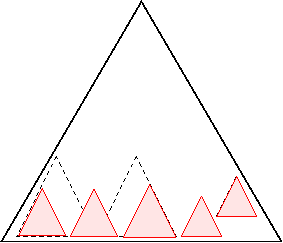
\includegraphics[width=.4\columnwidth]{images/granularity2}
    \caption{Schematic depiction of granularities.}
    \label{fig:granularity}
  \end{center}
\end{figure}

Granularities can, but do not have to be hierarchically structured. For example,
in text natural granularities are line, word or character. On the other
hand in more specialized content like a table one could distinguish
granularities like row, column, or cell, where the latter again can be
segmented by normal text granularities.  Defining a granularities is therefore
not necessarily a simple task in particular due to often heavily nesting of
layout elements in rich web applications.\ednote{Does that make sense?}


\subsection{Axis 2: Walking Content}
\label{sec:ax2}

Interactive navigation of content is accomplished by walkers.  They provide a
means to move between the different leaf nodes defined by a particular
granularity. They also offer the flexibility to break up the linear order of
navigating content as well as ignore certain leafs nodes. Fig.~\ref{fig:walkers} gives
an idea of different walkers operating on the same level of granularity.

The flexibility of the walkers is particular important to allow for a good user
experience on complex web content, where the ideal reading order is not
reflected by the order of the elements in the DOM. An example is the
\url{google.com} search page, which can contain in addition to the normal search
results additional information in the form of a knowledge card on the right or
timely information on the top (e.g., sports results). However, in the DOM the
knowledge card is given after all the search results, thus conventional linear
navigation would force the user to navigate through the entire list of search
results first before discovering the knowledge card.\ednote{Is that a good
  example?}

\begin{figure}[ht!]
  \begin{center}
    \leavevmode
    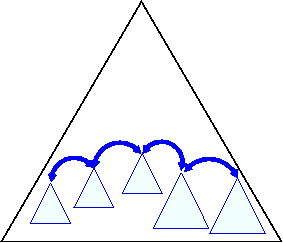
\includegraphics[width=.4\columnwidth]{images/walker1}
    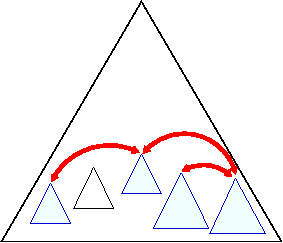
\includegraphics[width=.4\columnwidth]{images/walker2}
    \caption{Schematic depiction of different walkers.}
    \label{fig:walkers}
  \end{center}
\end{figure}

In practice walkers and granularities are exposed to the user in meaningful
combinations only. Walkers usually group related granularities, whenever
possible in a hierarchical nature.  A user can not only switch explicitly
between levels of granularity but interactively walk at one level of
granularity, while if necessary exploring the currently active leaf node at the
next lower level of granularity.

For example, in default text walking mode granularities include line, word and
character. The user can either switch between these granularities, or while
walking the text linearly, for instance, in line granularity --- usually with up
and down cursor keys\footnote{These keys depend on the particular choice of
  keymap and possible user customization.}  --- explore the content of the line
that currently being read word for word using the left and right cursor keys.

Immediate keyboard shortcuts can be given to particular combinations of walker
and granularity. A particular example is the exploration of hyperlinks in a
document to which ChromeVox dedicates two keys explicitly for walking links
only, while ignoring all interspersed text.

\subsection{Axis 3: Speech Output}
\label{sec:ax3}

The third axis along which ChromeVox is customizable is how speech output is
generated. While the way regular text is read is determined by the TTS engine
employed and thus can not be influenced by ChromeVox directly, when conveying
additional information on content as well as while reading specialized content
flexibility on how elements are spoken or announced is important.

For example, ChromeVox can provide the user with context information on
particular elements, such as announcing the type of headers, whether a hyperlink
is contained etc., by announcing the element explicitly or playing
earcons. Simple adaptations of this behavior allows for changes
\begin{inparaenum}[(a)]
\item to the level of verbosity,
\item if and how punctuation is being read,
\item to switch earcons on or off.
\end{inparaenum}

More complex structures can benefit from even more sophisticated customization.
For instance, when traversing tables ChromeVox can give the user information on
the current position in the table, for example, by announcing explicitly row and
column number or the cell type. Similarly, when speaking mathematics can become
necessary to alter the pronunciation of elements or entire formulas according to
mathematical subject area or user preference.

For this purpose ChromeVox has a dedicated speech rule engine that allows to
specify speech rules for particular DOM element. If a walker traverses a DOM
element for which a speech rule exists, it is used to generate speech
output. This can be a recursive process in the sense the execution of one speech
rule might trigger further speech rules that apply to its sub-elements.
Customization is realized by defining different rules for elements and
parameterizing the engine swapping entire rule sets thus changing the generated
speech output.

As ChromeVox's speech rule engine has been designed originally in the context of
our work on making mathematics accessible we shall present more details on its
operation in Sec.~\ref{sec:translate}. However, it has now been integrated as a
general component in the screen reader and can be employed to customize reading
of any element in the DOM.

\subsection{Axis 4: Alternative Representations}
\label{sec:ax4}


The final axis of customization is ChromeVox's ability to swap entire elements
in the DOM for alternative representations. However, as we do not want to alter
the actual DOM, we achieve this by internally mapping particular leaf node to
dedicated representations. This idea is schematically depicted in
Fig.~\ref{fig:alt}.

\begin{figure}[ht!]
  \begin{center}
    \leavevmode
    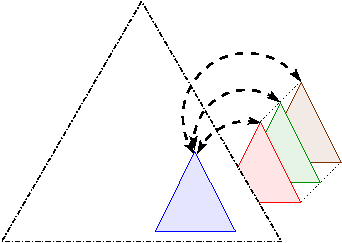
\includegraphics[width=.5\columnwidth]{images/substructure1}
    \caption{Schematic depiction of alternative representations.}
    \label{fig:alt}
  \end{center}
\end{figure}

The use of alternative representations can be particularly useful when the
original DOM element is not suitable for speech generation or when a more
dedicated data structure can give lead to a better understanding of the content
for the user. In fact, this ability plays a crucial role in the accessibility of
mathematical content and we describe it in more detail in Sec.~\ref{sec:alternative}.

\section{Speaking Mathematics}
\label{sec:translate}

\begin{description}
\item[Continuously] 
\item[In interactive granularities] 
\end{description}

Embedded in regular text maths expressions are treated as leaf nodes, that is

\section{Rerepresenting Maths Content}
\label{sec:alternative}



\section{Engaging with Content}
\label{sec:explore}

We consider the example 

\begin{equation}
x_1^2+x_2 = y\label{eq:simple}
\end{equation}

Tree exploration:

\tabcolsep1pt
\noindent\begin{tabular}{clclcl}
& $\framebox{$x_1^2+x_2 = y$}$ & $\longleftrightarrow$ 
$\framebox{$x_1^2$}+x_2 = y$ & $\longleftrightarrow$ 
$\framebox{x}_1^2+x_2 = y$ \\ 
$\longleftrightarrow$  & 
$x_{\framebox{$1$}}^2+x_2 = y$ & $\longleftrightarrow$ 
$x_1^{\framebox{$2$}}+x_2 = y$ & $\longleftrightarrow$ 
$x_1^2\framebox{$+$}x_2 = y$\\
$\longleftrightarrow$  & 
$x_1^2+\framebox{$x_2$} = y$ & $\longleftrightarrow$ 
$x_1^2+\framebox{$x$}_2 = y$ & $\longleftrightarrow$ 
$x_1^2+x_{\framebox{$2$}} = y$ \\
$\longleftrightarrow$  & 
$x_1^2+x_2\framebox{$=$}  y$ & $\longleftrightarrow$ 
$x_1^2+x_2 = \framebox{$y$}$ 
\end{tabular}

Level exploration:

\tabcolsep2pt
\noindent\begin{tabular}{lclcl}
Level 0 & & Level 1 & & Level 2\\
$\framebox{$x_1^2+x_2 = y$}$ 
& $\longleftrightarrow$ &
$\framebox{$x_1^2$}+x_2 = y$ 
& $\longleftrightarrow$ &
$\framebox{$x$}_1^2+x_2 = y$ \\
& & & & $x_{\framebox{$1$}}^2+x_2 = y$ \\
& & & & $x_1^{\framebox{$2$}}+x_2 = y$ \\
& & $x_1^2\framebox{$+$}x_2 = y$  \\
& & $x_1^2+\framebox{$x_2$} = y$  
& $\longleftrightarrow$ &
$x_1^2+\framebox{$x$}_2 = y$\\
& & & & $x_1^2+x_{\framebox{$2$}} = y$\\
& & $x_1^2+x_2\framebox{$=$}  y$\\
& & $x_1^2+x_2 = \framebox{$y$}$\\
\end{tabular}









\section{Conclusions}
\label{sec:conc}


\bibliographystyle{plain} \bibliography{www_2014}

\end{document}
